\begin{IEEEbiography}[{
\includegraphics[width=1in,height=1.25in,clip,keepaspectratio]{Images/a1.png}}]
    {Stamatios Orfanos} is a Ph.D. candidate in Digital Systems, University of Piraeus, Greece, where he specializes in computer vision, 
    reinforcement learning, data analysis and wearable healthcare systems. He holds a B.Sc. in Computer Science and Telecommunications and an M.Sc. 
    in Artificial Intelligence from National Research Center Demokritos and University of Piraeus. As an AI Architect and Engineer in Bioassist, he leads the 
    design and implementation of AI-driven systems, on many different fields and applications. His current research centers on developing lightweight
    machine learning algorithms for wearable sensors to support remote patient monitoring and adaptive rehabilitation.
    Mr. Orfanos is a member of IEEE and actively collaborates with clinical partners to translate his research into real-world applications.
\end{IEEEbiography}

\begin{IEEEbiography}[{
\includegraphics[width=1in,height=1.25in,clip,keepaspectratio]{Images/a2.jpg}}]
    {THANITA SANGHAN} received the B.Sc. degree in Thai traditional medicine from the Faculty of Traditional Thai Medicine, Prince of Songkla 
    University, in 2009, and the M.Sc. degree in biomedical engineering from the Faculty of Medicine, in 2012. She is currently pursuing the Ph.D.
    degree in biomedical engineering with the Faculty of Medicine, Prince of Songkla University. Her research interests include gait analysis, gait 
    biomechanics, hemiplegic gait, and stroke rehabilitation. She is also involved in a Horizon Europe: gaitREHub Project focused on developing 
    intelligent wearable system for enhanced personalized gait rehabilitation.
\end{IEEEbiography}

\begin{IEEEbiography}[{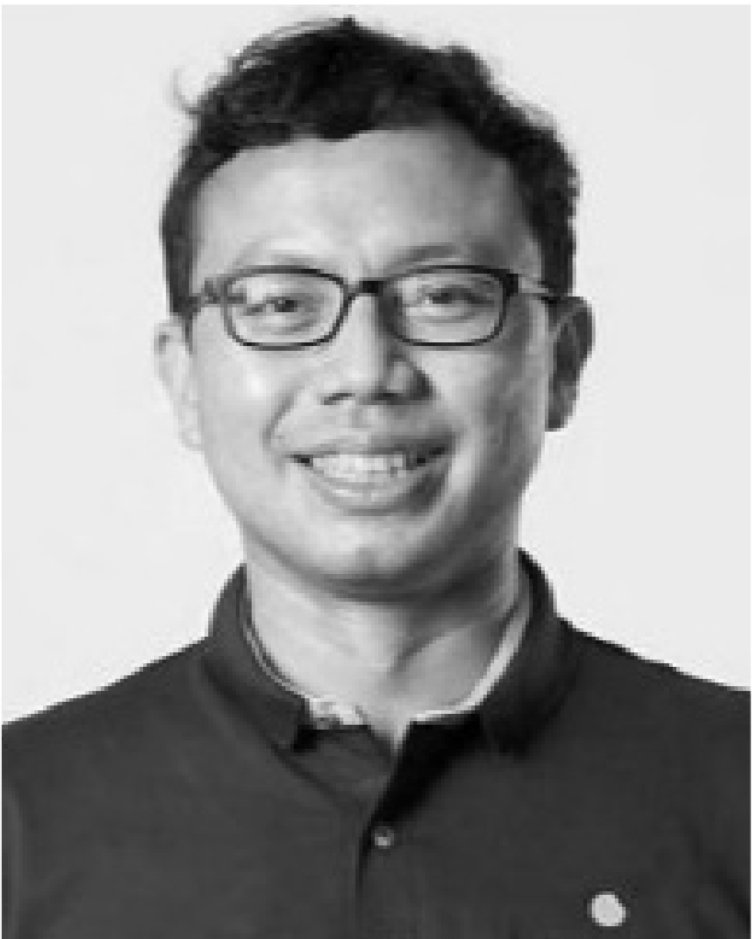
\includegraphics[width=1in,height=1.25in,clip,keepaspectratio]{Images/a3.jpg}}]
    {SURAPONG CHATPUN} received the B.Eng. degree in mechanical engineering from Chulalongkorn University, Thailand, in 1996, and the M.Eng. 
    degree from the University of Tokyo,Japan, in 2003, and the Ph.D. degree in bioengineering from the University of California, USA,
    in 2010. He currently leads the Cardiovascular Engineering Research Laboratory (CERLab) at the Faculty of Medicine, Prince of Songkla 
    University. His research interests include applying engineering approaches, such as continuum mechanics, numerical methods (e.g.FEM), 
    fluid mechanics (e.g. CFD), image processing and computer-aided design, combined with life sciences knowledge and available technologies
    to enhance understanding of circulatory system’s function and mechanisms in both normal and pathological conditions. He also designs and invents
    medical devices not only for cardiovascular applications but also for other clinical areas, such as rehabilitation and orthopedics. He is also 
    coordinating a Horizon Europe: gaitREHub project in the field of the intelligent wearable system for enhanced personalized gait rehabilitation.
\end{IEEEbiography}

\begin{IEEEbiography}[{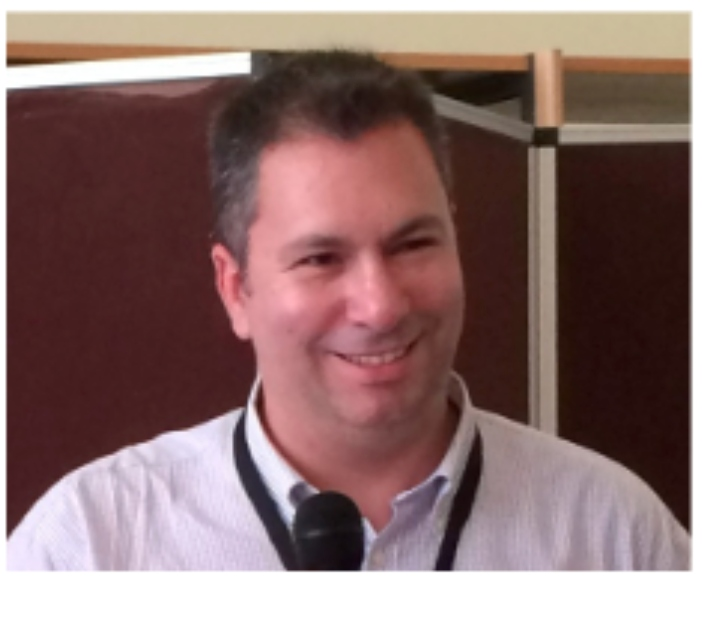
\includegraphics[width=1in,height=1.25in,clip,keepaspectratio]{Images/a4.jpg}}]
    {ANDREAS MENYCHTAS} 
\end{IEEEbiography}

\begin{IEEEbiography}[{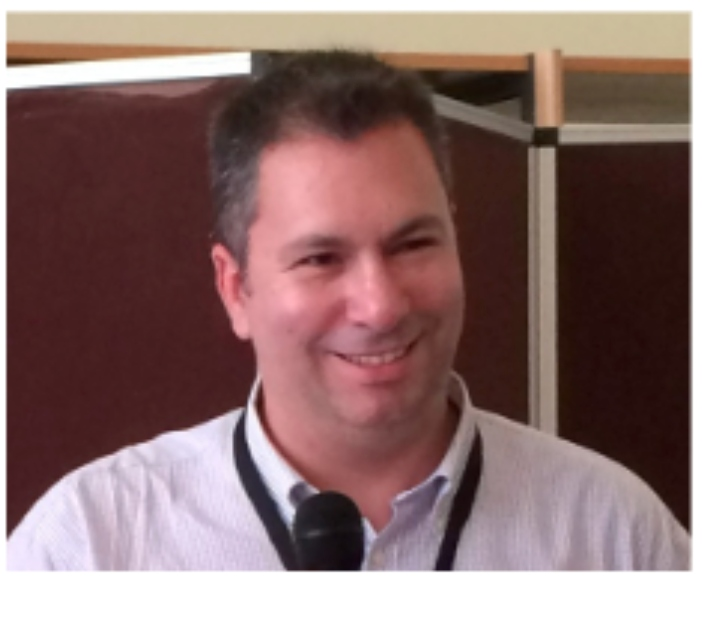
\includegraphics[width=1in,height=1.25in,clip,keepaspectratio]{Images/a4.jpg}}]
    {CHRISTOS PANAGOPOULOS} 
\end{IEEEbiography}

\begin{IEEEbiography}[{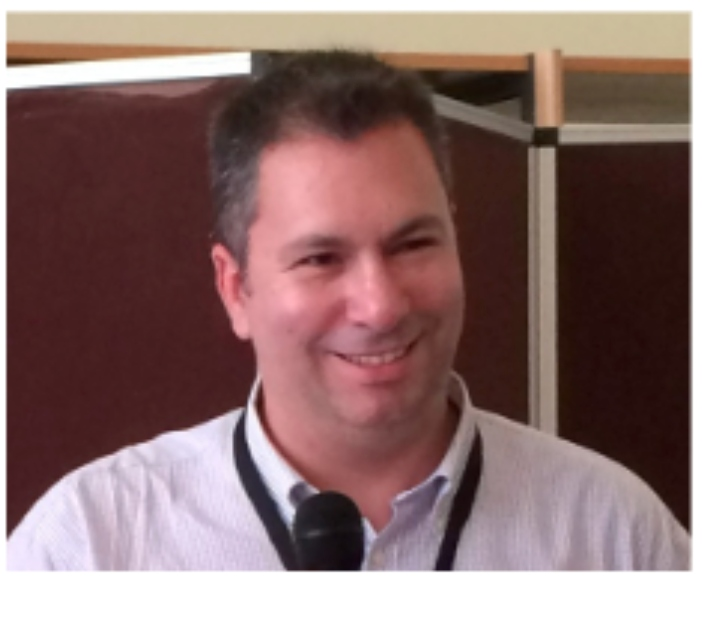
\includegraphics[width=1in,height=1.25in,clip,keepaspectratio]{Images/a4.jpg}}]
    {ILIAS MAGLOGIANNIS} (M'00-SM'11) re-ceived a Diploma in Electrical \& Computer Engineering and a Ph.D. in Biomedical Engineering and Medical 
    Informatics from the National Technical University of Athens (NTUA). He is now Professor and Director of the Computational Biomedicine 
    Laboratory in the Dept. of Digital Systems in the University of Piraeus. His scientific interests include Biomedical Informatics, 
    Computer Vision, AI, Multimedia Processing and Pervasive Healthcare Systems. He has been engaged as principal investigator in many European and 
    National Research programs. His published scientific work includes five (5) books and more than 400 journal and conference papers, while has 
    received more than 8200 citations on his published work. He is a senior member of the IEEE, ACM, SPIE, president of IFIP Working Group WG12.5 
    (AI Applications) and vice president of IEEE EMBS Greek chapter.
\end{IEEEbiography}
